% This is samplepaper.tex, a sample chapter demonstrating the
% LLNCS macro package for Springer Computer Science proceedings;
% Version 2.20 of 2018/03/10
%
\documentclass[runningheads]{llncs}

\usepackage[T1]{fontenc}
\def\doi#1{\href{https://doi.org/\detokenize{#1}}{\url{https://doi.org/\detokenize{#1}}}}
%
\usepackage{graphicx}
% Used for displaying a sample figure. If possible, figure files should
% be included in EPS format.
%
% If you use the hyperref package, please uncomment the following line
% to display URLs in blue roman font according to Springer's eBook style:
% \renewcommand\UrlFont{\color{blue}\rmfamily}
%
\usepackage{subcaption}
\usepackage{listings}
\lstset{language=Pascal}
% Please use the

\begin{document}
%
\title{ENTAILMENT IN LANGUAGE PRAGMATICS\thanks{}}
%
%\titlerunning{Abbreviated paper title}
% If the paper title is too long for the running head, you can set
% an abbreviated paper title here
%
\author{SAINEY MANGA}
%
\authorrunning{Sainey Manga}
% First names are abbreviated in the running head.
% If there are more than two authors, 'et al.' is used.
%
\institute{University of Milan, Milan, Italy\\
\email{sainey.manga@studenti.unimi.it}}
%
\maketitle              % typeset the header of the contribution
%
%\begin{abstract}


\keywords{Textual Entailment  \and Premise \and Hypothesis.}
%\end{abstract}
%
%
%
\section{INTRODUCTION}
Text Entailment (TE) or Natural Language Inference (NLI) is defined as a relation between two natural language sentences (a text P and a hypothesis H) that holds if a human reading P would infer that H is most likely true. The study of the relationship between two pieces of text deals with deriving whether one implies the meaning of another. It is regarded as the basic step towards natural language understanding, but extremely challenging due to the natural complexity of human languages. A common phenomenon is that there exist a lot of ways to express the same or similar meaning. To discover such different expressions, the TE task is proposed to judge whether the meaning of the hypothesis can be inferred (entailed) from the premise. Understanding the semantic relationship between two sentences is a key for improving performance in several NLP tasks such as Automatic Text Summarization, Question and Answering, Machine Translation etc. 
\begin{table}
	\caption{Textual Entailment Examples}\label{tab1}
	\begin{tabular}{|l|l|l|}
		\hline
		 {\Large\bfseries Premise} &  {\Large\bfseries Hypothesis} &  {\Large\bfseries Label}\\
		\hline
		A person on a horse jumps over a broken down airplane &  A person is at a dine, 
		ordering an omelette
& contradiction\\
		Two women are embracing while holding to go packages. &  Two women are holding 

		packages.
& entailment\\
		Children smiling and waving at camera &They are smiling at their parents &neutral\\
		\hline
	\end{tabular}
\end{table}
There have been promising developments in NLP with several investigations of approaches focusing on TE in the literature. These models include models based on lexical similarities, models based on formal reasoning, Feature-based models, Sentence vector-based models,
and most recently deep neural models.  Some methods use statistical classifiers which leverage a wide variety of features, including hand-engineered features derived from complex NLP pipelines
and similarity between sentences (P and H) and sentence pairs ((P',H') and (P'',H'')); (Malakasiotis and Androutsopoulos, 2007; Jijkoun and de Rijke, 2005; Wan et al., 2006; Zanzotto and Moschitti, 2006) extract the structured information in P -H pair and check if the information in P contains or can infer the information in H. For the neural network-based methods, (Bowman et al., 2015), Rocktaschel et al. (2015) used the attention-based technique to improve the performance of LSTM-based recurrent neural network. P. Parikh et al (2016) used attention to decompose the problem into subproblems that can be solved separately, thus making it trivially parallelizable.
The goal of this project is to define models that detect possible entailments given an input utterance. The models would be able to infer if the given sentence (Hypothesis) is an entailment to another sentence (premise) or not. To achieve this goal, I implemented a Decomposable attention model (DAM) based on P. Parikh et al (2016) and compared it with two traditional machine learning models.
\section{RESEARCH QUESTION AND METHODOLOGY}
\subsubsection{Research Question} The main research question of this project is to predict what
the label is given two sentences. That is to say, is the hypothesis an entailment, contradiction or neutral to the premise sentence? The project will further investigate and compare which model has the best performance.

\subsubsection{Methodology} {:}To achieve the goals above, the DAM model was implemented as well the Logistic Regression model and the Naïve Bayes Classifier.
	\begin{itemize}
		\item•	DAM Model: This approach was implemented by P. Parikh et al (2016), where they have argued that for natural language inference, it can often suffice to simply align bits of local text substructure and then aggregate this information. They first created a soft alignment matrix using neural attention based on Bahdanau et al (2015), then used the (soft) alignment to decompose the task into subproblems that are solved separately. Finally, the results of these subproblems were merged to produce the final classification. In addition, they optionally applied intra-sentence attention based on Cheng et al (2016) to endow the model with a richer encoding of substructures prior to the alignment step. Asymptotically, their approach does the same total work as a vanilla LSTM encoder, while being trivially parallelizable across sentence length, which can allow for considerable speedups in low-latency settings.  See the structure of the achitecture in Figure 1.
\\
		\\
		\begin{figure}
			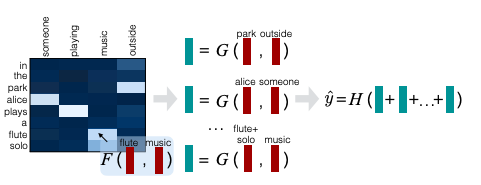
\includegraphics[scale=0.8]{model achitect}
			\centering
			\caption{Pictorial overview of the DAM, showing the Attend (left), Compare (center) and Aggregate (right) steps.\\
			The architecture is taken from the published paper.}
			\label{fig:dataset}
		\end{figure}
			\item •	Logistic Regression: falls in a class of probabilistic models referred to as discriminative models. Such models assume that the dependent variable is an observed value generated from a probabilistic distribution defined by a function of the feature variables. \\
			\item •	Naive Bayes Classifier: uses a probabilistic generative model that is identical to the mixture model used for clustering. The model assumes that the corpus is generated from a mixture of different classes. The observed (training and test) data are assumed to be outcomes of this generative process, and the parameters of this generating process are estimated so that the log- likelihood of this data set being created by the generative process is maximized. 
		\end{itemize}

% \paragraph{Sample Heading (Fourth Level)}
%	The contribution should contain no more than four levels of
%	headings. Table~\ref{tab1} gives a summary of all heading levels.
\section{EXPERIMENTAL RESULTS}
\subsubsection{Data Description}
The dataset used in this project is The Stanford Natural Language Inference (SNLI) corpus (version 1.0). It is a collection of 570k human-written English sentence pairs manually labeled for balanced classification with the labels entailment, contradiction, and neutral. These labels defined the relationship between the sentence pairs. The label represents the majority of vote by the annotators’ judgement. The dataset is divided in to separate training set with about 550,000 observations, validation set with about 10,000 observations and a test set of about 10,000 observations. It contains 10 attributes in total, but our interest lies only in three attributes namely; sentence1 which we will refer to as Premise, sentence2 which we refer to as Hypothesis, and Gold-label which we will refer to simply as Label. There are no missing values for the dataset stored under Jason files, which we utilized.\\   
	\\
\begin{figure}
	\begin{subfigure}{.5\textwidth}
		\centering
		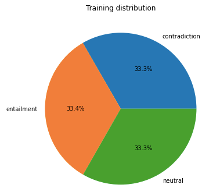
\includegraphics[width=1\linewidth]{hist.png}  
		\label{fig:sub-first}
	\end{subfigure}
	\begin{subfigure}{.5\textwidth}
		\centering
		% include second image
		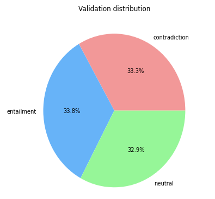
\includegraphics[width=1\linewidth]{hist1.png}  
		%\caption{Put your sub-caption here}
		\label{fig:sub-second}
	\end{subfigure}
	\caption{DATA DISTRIBUTION}
	\label{fig:fig}
\end{figure}


Figure 2 shows that both our data sets are balance between the three labels. The training data is more balance with each label containing 33\% of the data. The validation data on the other hand has a distribution of about 34\% for entailment and 33\% for each of the other two labels.\\
\\
\begin{figure}
	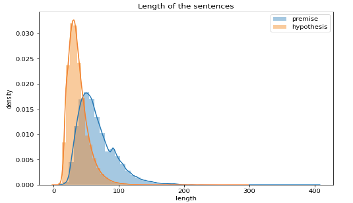
\includegraphics[scale=1]{lensen.png}
	\centering
	\caption{Length of sentence in each attribute}
	\label{fig:dataset}
\end{figure}
In Figure 3, we can see that most of the sentences in the hypothesis have length between 20 to 70 and that there are no sentences with a length more than hundred. In the premise, most sentences have a length between 60 to 90 and that few sentences have a length above hundred.\\
\\
\begin{figure}
	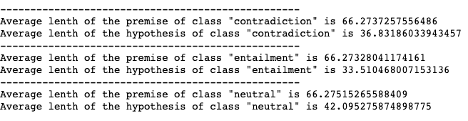
\includegraphics[scale=0.8]{avesenlen.png}
	\centering
	\caption{Average length of sentence in each label}
	\label{fig:dataset}
\end{figure}
In Figure 4, For the premise, the average length of sentences for all the labels is about 66 for all the data sets. On the other hand, the average length of sentences in the hypothesis labeled as contradiction is about 37, about 34 for the label entailment, and 42 for the label neutral. We therefore choose to visualize the length of sentences in each label in the hypothesis.\\
\\
\begin{figure}
	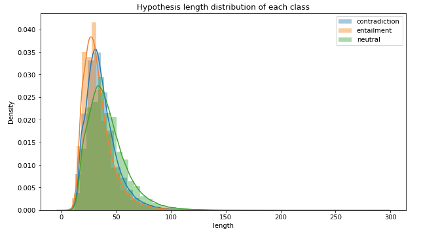
\includegraphics[scale=0.8]{hypsenlen.png}
	\centering
	\caption{:Length of sentences in label of hypothesis}
	\label{fig:dataset}
\end{figure}
From Figure 5, most of the sentences in each of the labels in the hypothesis have a length ranging between 20 to 60, although the labels neutral and contradiction have more sentences distributed above 60 than the entailment label.
\subsubsection{Metrics For Evaluation}{:}
Confusion Matrix was used to evaluate the performances of our various models. It is a specific table layout that allows visualization of the performance of an algorithm. Each row of the matrix represents the instances in an actual class while each column represents the instances in a predicted class, or vice versa – both variants are found in the literature. The name stems from the fact that it makes it easy to see whether the system is confusing two classes.
\subsubsection{Experimental Methodology}
\begin{itemize}
\item •	Data Cleaning {:} The data set was first cleaned by removing punctuation marks and other unwanted characters as well as setting all the text to lowercase. During the data annotation, a label which could not have a single majority has an {“underscore”} as a placeholder, so we completely disregarded those instances in our dataset. 

\item •	Feature Engineering{:}Since the labels contain three classes, indexing was used to encode these classes into indexes of 0, 1 and 2.  From indexing the classes, a text tokenization was implemented using TensorFlow. A word index was generated when applied to the concatenated training and validation texts. Using the tokenizer, sentences are converted into sequences with each word having its unique index. To make so that inputs have the same shape, a max sequence length was determined, and zeros were appended to the sequence vectors until their length matches the max. The max length of the sequence was set at 50. The final stage of data organization for the DAM model is setting the embedding model. Pre-trained embeddings were used to ensure better word representations. The data  word2vec-google-news-300 in gensim was used.
\\
For the purpose of the Machine Learning Models, a separate vectorization was implemented using TF-IDF vectorizer. This was easily done using sklearn functions.
\item •	Model Implementation{:}The DAM model was implemented using Keras with TensorFlow, and Sklearn was used to implement both the Logistic Regression and the Naïve Bayes classifier.\\
The layers that were defined to model the DAM architecture composed of 3 main steps as we have seen in figure 1. The first step called Attend, finds word-level alignments between sentences by computing pairwise similarity and soft-alignment. To compute pairwise similarity, the embedded representations of sequences are passed through a feed-forward network (FFN) to yield non- linear transformations. The FFN uses 2 hidden layers each with 200 nodes and ReLU activations. Dropout layers with a dropout rate of 0.1 were also added in-between layers to regularize the network and help prevent over-fitting. Vector similarities are then computed using the non-linear outputs and passing these through a dot product layer. The similarities are normalized to carry out soft-alignment and the result along with the target embeddings are put through a further dot product layer. The results from these generate α which is the sub-phrase in the premise that is softly aligned with the hypotheses and vice versa for β. The second Compare step concatenates the previous results with the embeddings of the target sequences and passes the concatenated result through a further FFN to achieve the comparison vectors v1 and v2. The third Aggregate step aggregates each of the vectors and concatenates both results together.  A final FFN receives the concatenated result as input and applies its output to a dense layer of 3 nodes with SoftMax activation for outputting the model’s predictions. Epochs were set to 20 with a batch size of 512.
\\
The Logistic model was set with a maximum iteration of 2000 and a multiclass as 'ovr'.  The Naïve Bayes was also simply defined through Sklearn

\end{itemize}
\subsubsection{Experimental Results} {:}
\\
\begin{table}
\begin{center}
	\caption{Results of various models.
	tables}\label{table:2}
	\begin{tabular}{||c c c c||} 
		\hline
		MODEL & TRAINING ACCURACY & VALIDATION ACCURACY &TESTING ACCURACY \\ [0.5ex] 
		\hline\hline
	DAM MODEL & 0.8600 &0.8455&    0.8491 \\ 
		\hline
	LOGISTIC REG. &0.7244 &   -      &        0.6337 \\
		\hline
	NAÏVE BAYES &   0.6266 &  -      &       0.6318 \\
		\hline
	\end{tabular}
\end{center}
\end{table}
In Table 2, we can clearly see that the DAM model provides much better accuracy than the Machine Learning Models we implemented.  However, our DAM model has underperformed compared to the original model implemented by P. Parikh et al (2016). Their model had a training and testing accuracy of 89.5 and 86.3 respectively.

As we can see in the confusion matrices in Figure 6, the DAM model has less false positives in each of the label classes than the two machine learning models. Both the logistic and the Naïve bayes models provide somewhat similar results. In all the models, there was more miss-matched in the neutral label than the other two models.

\\
\begin{figure}[ht]
	\subfloat[DAM model]{
		\begin{minipage}[c][1\width]{
				0.3\textwidth}
			\centering
			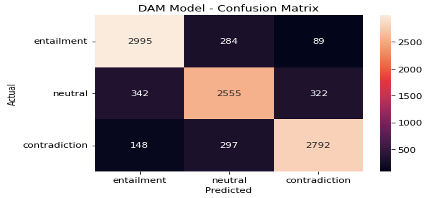
\includegraphics[width=1.5\textwidth]{matrix1.png}
	\end{minipage}}
	\hfill 	
	\subfloat[LG]{
		\begin{minipage}[c][1\width]{
				0.3\textwidth}
			\centering
			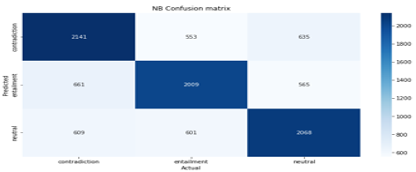
\includegraphics[width=1.5\textwidth]{matrix2.png}
	\end{minipage}}
	\hfill	
	\subfloat[NB]{
		\begin{minipage}[c][1\width]{
				0.3\textwidth}
			\centering
			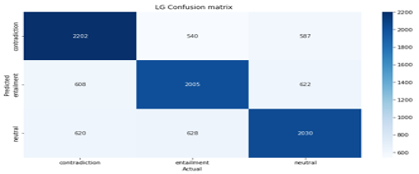
\includegraphics[width=1.8\textwidth]{matrix3.png}
	\end{minipage}}
	\caption{Confusion Matrices }
\end{figure}

\section{CONCLUSION}
TE or NLI is an interesting yet challenging task in NLP. The project implemented a DAM model based on the original model of the P. Parikh et al (2016), then implemented two machine learning models. Our DAM model’s accuracy somewhat underperformed the adopted model but outperformed the two counterparts’ models. However, the result of our model is consistent with the state-of-the-art results. As can be seen in the results of Bowman et al. (2016), Yang Liu et al. (2016), Conneau et al. (2017) etc. In the future it would be of interest to add an LSTM layer to the DAM model to see if it would improve the result.



%\noindent Displayed equations are centered and set on a separate
%line.
%\begin{equation}
%x + y = z
%\end{equation}
%Please try to avoid rasterized images for line-art diagrams and
%schemas. Whenever possible, use vector graphics instead (see
%Fig.~\ref{fig1}).

%\begin{figure}
%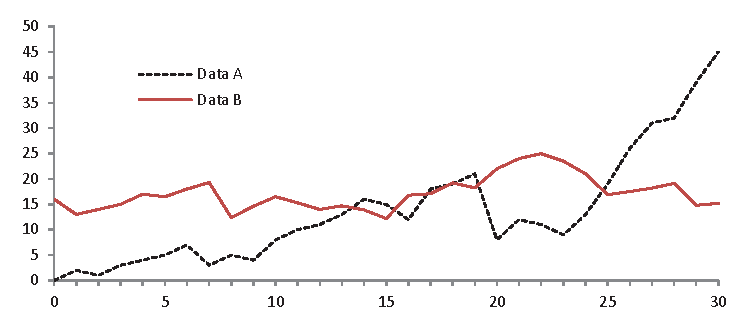
\includegraphics[width=\textwidth]{fig1.eps}
%\caption{A figure caption is always placed below the illustration.
%Please note that short captions are centered, while long ones are
%justified by the macro package automatically.} \label{fig1}
%\end{figure}

%Program listings or code snippets in the text like \lstinline!var i:integer;!
%should be set in typewriter font. The ``listings'' macro package can be used
%for reader-friendly syntax highlighting as in the following Pascal sample code:\footnote{For
%typesetting pseudocode, the ``algorithmic'', ``algorithm2e'', ``algorithmicx'',
%and ``program'' packages are also worth considering.}
%\begin{lstlisting}
%for i:=maxint to 0 do
%begin
   % { do nothing }
%end;
%Write('end of sample code');
%\end{lstlisting}


%\begin{theorem}
%This is a sample theorem. The run-in heading is set in bold, while
%the following text appears in italics. Definitions, lemmas,
%propositions, and corollaries are styled the same way.
%\end{theorem}
%
% the environments 'definition', 'lemma', 'proposition', 'corollary',
% 'remark', and 'example' are defined in the LLNCS documentclass as well.
%
%\begin{proof}
%Proofs, examples, and remarks have the initial word in italics,
%while the following text appears in normal font.
%\end{proof}
%For citations of references, we prefer the use of square brackets
%and consecutive numbers. Citations using labels or the author/year
%convention are also acceptable. The following bibliography provides
%a sample reference list with entries for journal
%articles~\cite{ref_article1}, an LNCS chapter~\cite{ref_lncs1}, a
%book~\cite{ref_book1}, proceedings without editors~\cite{ref_proc1},
%and a homepage~\cite{ref_url1}. Multiple citations are grouped
%\cite{ref_article1,ref_lncs1,ref_book1},
%\cite{ref_article1,ref_book1,ref_proc1,ref_url1}.

%\subsubsection{Acknowledgements} Please place your acknowledgments at
%the end of the paper, preceded by an unnumbered run-in heading (i.e.
%3rd-level heading).


%
% ---- Bibliography ----
%
% BibTeX users should specify bibliography style 'splncs04'.
% References will then be sorted and formatted in the correct style.
%
% \bibliographystyle{splncs04}
% \bibliography{mybibliography}
%

\begin{thebibliography}{8}
\bibitem{ref_article1}
Parikh, Ankur P., et al. : A Decomposable Attention Model for Natural Language Inference.  arXiv preprint arXiv: \textbf1606.01933  (2016)

\bibitem{ref_lncs1}
Ryan Camilleri: Applying Recurrent Layers to the Decomposable Attention Model for Natural Language Inference. University of Malta

\bibitem{ref_article1}
Poliak, A : A survey on recognizing textual entailment as an nlp evaluation. arXiv preprint: \textbf  (2020)
\bibitem{ref_article1}
Bowman, Samuel R., et al. : A large annotated corpus for learning natural language inference.  arXiv preprint arXiv: \textbf1508.05326  (2015)
%\bibitem{ref_book1}
%Author, F., Author, S., Author, T.: Book title. 2nd edn. Publisher,
%Location (1999)

%\bibitem{ref_proc1}
%Author, A.-B.: Contribution title. In: 9th International Proceedings
%on Proceedings, pp. 1--2. Publisher, Location (2010)

%\bibitem{ref_url1}
%LNCS Homepage, \url{http://www.springer.com/lncs}. Last accessed 4
%Oct 2017
\end{thebibliography}
\end{document}
